% MIT License:
%
% Copyright 2021 Sathvik Srinivas
%
% Permission is hereby granted, free of charge, to any person obtaining a copy of this software and associated documentation files (the "Software"), to deal in the Software without restriction, including without limitation the rights to use, copy, modify, merge, publish, distribute, sublicense, and/or sell copies of the Software, and to permit persons to whom the Software is furnished to do so, subject to the following conditions:
%
% The above copyright notice and this permission notice shall be included in all copies or substantial portions of the Software.
%
% THE SOFTWARE IS PROVIDED "AS IS", WITHOUT WARRANTY OF ANY KIND, EXPRESS OR IMPLIED, INCLUDING BUT NOT LIMITED TO THE WARRANTIES OF MERCHANTABILITY, FITNESS FOR A PARTICULAR PURPOSE AND NONINFRINGEMENT. IN NO EVENT SHALL THE AUTHORS OR COPYRIGHT HOLDERS BE LIABLE FOR ANY CLAIM, DAMAGES OR OTHER LIABILITY, WHETHER IN AN ACTION OF CONTRACT, TORT OR OTHERWISE, ARISING FROM, OUT OF OR IN CONNECTION WITH THE SOFTWARE OR THE USE OR OTHER DEALINGS IN THE SOFTWARE.

\documentclass[12pt]{article}

\usepackage{amsmath}
% change compiler to XeLaTeX in overleaf settings
\usepackage{fontspec}


\usepackage[a4paper, left=1in, right=1in, top=1.2in, bottom=1in, headsep=0.6in]{geometry}
\usepackage[nottoc]{tocbibind}
\usepackage{fancyvrb}
\usepackage{float}
\usepackage{caption}
\usepackage{boldline}
\usepackage{tabularx,colortbl}
\usepackage{graphbox}
\usepackage{lipsum}
\usepackage{subcaption}
\usepackage{enumerate}
\usepackage[bottom]{footmisc}
\usepackage{array}
\usepackage{diagbox}


\usepackage{titlesec}


\newcommand\mysectionsize{\fontsize{18pt}{12pt}\selectfont}
\newcommand\mysubsectionsize{\fontsize{16pt}{10pt}\selectfont}
\newcommand\mysubsubsectionsize{\fontsize{14pt}{7pt}\selectfont}

\titleformat{\section}
{\normalfont\mysectionsize\bfseries}{\thesection}{1em}{}
\titleformat{\subsection}
{\normalfont\mysubsectionsize\bfseries}{\thesubsection}{1em}{}
\titleformat{\subsubsection}
{\normalfont\mysubsubsectionsize\bfseries}{\thesubsubsection}{1em}{}

\usepackage{chngcntr}
\counterwithin{figure}{section}

\renewcommand{\thefootnote}{\fnsymbol{footnote}}
\usepackage{graphicx}
\usepackage{tikz}
\usetikzlibrary{calc}
\usetikzlibrary{decorations.pathmorphing}

\usepackage{tocloft}




\usepackage{listings}
% the below three commands need to be renewed as required
% see Figure 3. for example
% this command makes the figure name start with "Figure <section number>.<table alphabet>"
\renewcommand{\thefigure}{\arabic{section}(\alph{figure})}
% this command makes the figure name start with "Figure <section number>.<subsection>.<table alphabet>"
\renewcommand{\thefigure}{\arabic{section}.\arabic{subsection}(\alph{figure})}
% this command makes the figure name start with "Figure <section number>.<subsection>.<subsubsection>.<table alphabet>"
\renewcommand{\thefigure}{\arabic{section}.\arabic{subsection}.\arabic{subsubsection}(\alph{figure})}

\setcounter{figure}{0}

\renewcommand{\thetable}{\arabic{section}(\alph{table})}
\renewcommand{\thetable}{\arabic{section}.\arabic{subsection}(\alph{table})}
\renewcommand{\thetable}{\arabic{section}.\arabic{subsection}.\arabic{subsubsection}(\alph{table})}

\setmainfont{Times New Roman}
\usepackage{xcolor}
\definecolor{codegreen}{rgb}{0,0.6,0}
\definecolor{codegray}{rgb}{0.5,0.5,0.5}
\definecolor{codepurple}{rgb}{0.58,0,0.82}
\definecolor{backcolour}{rgb}{0.95,0.95,0.92}
\definecolor{anti-flashwhite}{rgb}{0.95, 0.95, 0.96}
\definecolor{crimsonglory}{rgb}{0.75, 0.0, 0.2}
\definecolor{ceruleanblue}{rgb}{0.16, 0.32, 0.75}

\lstset
{
    columns=fullflexible,
    breaklines=true,
    postbreak=\mbox{\textcolor{ceruleanblue}{$\hookrightarrow$}\space},
}
\lstdefinestyle{mystyle}{
    backgroundcolor=\color{anti-flashwhite},   
    commentstyle=\color{codegray},
    keywordstyle=\color{codegreen},
    numberstyle=\tiny\color{codegray},
    stringstyle=\color{crimsonglory},
    basicstyle=\ttfamily\footnotesize,
    breakatwhitespace=false,         
    breaklines=true,                 
    captionpos=b,                    
    keepspaces=true,                 
    numbers=left,                    
    numbersep=5pt,                  
    showspaces=false,                
    showstringspaces=false,
    showtabs=false,                  
    tabsize=2
}

\usepackage{color}   %May be necessary if you want to color links
\usepackage{setspace}
\usepackage{hyperref}
\hypersetup{
    colorlinks=true, %set true if you want colored links
    linktoc=all,     %set to all if you want both sections and subsections linked
    linkcolor=black,  %choose some color if you want links to stand out
    citecolor=black,
    urlcolor=black
}

\usepackage{fancyhdr}

\lstset{style=mystyle}


\cftsetindents{figure}{0em}{3.5em}
\cftsetindents{table}{0em}{3.9em}

%required for increasing nesting depth
\titleclass{\subsubsubsection}{straight}[\subsection]

\newcounter{subsubsubsection}[subsubsection]
\renewcommand\thesubsubsubsection{\thesubsubsection.\arabic{subsubsubsection}}
\renewcommand\theparagraph{\thesubsubsubsection.\arabic{paragraph}} % optional; useful if paragraphs are to be numbered
\titleformat{\subsubsubsection}
  {\normalfont\normalsize\bfseries}{\thesubsubsubsection}{1em}{}
\titlespacing*{\subsubsubsection}
{0pt}{3.25ex plus 1ex minus .2ex}{1.5ex plus .2ex}
\makeatletter
\renewcommand\paragraph{\@startsection{paragraph}{5}{\z@}%
  {3.25ex \@plus1ex \@minus.2ex}%
  {-1em}%
  {\normalfont\normalsize\bfseries}}
\renewcommand\subparagraph{\@startsection{subparagraph}{6}{\parindent}%
  {3.25ex \@plus1ex \@minus .2ex}%
  {-1em}%
  {\normalfont\normalsize\bfseries}}
\def\toclevel@subsubsubsection{4}
\def\toclevel@paragraph{5}
\def\toclevel@paragraph{6}
\def\l@subsubsubsection{\@dottedtocline{4}{7em}{4em}}
\def\l@paragraph{\@dottedtocline{5}{10em}{5em}}
\def\l@subparagraph{\@dottedtocline{6}{14em}{6em}}
\makeatother

\setcounter{secnumdepth}{4}
\setcounter{tocdepth}{4}

\usepackage{color, colortbl}
\definecolor{Gray}{gray}{0.9}

\usepackage{chngcntr}
\counterwithin{figure}{section}
\counterwithin{table}{section}

\begin{document}

% \maketitle

\begin{titlepage}
\newgeometry{right=0.9in,left=0.9in, top=0.9in, bottom=0.9in}
    \centering
\begin{tikzpicture}[overlay,remember picture]
    \draw [line width=1.4mm, decorate]
        ($ (current page.north west) + (0.85in,-0.85in) $)
        rectangle
        ($ (current page.south east) + (-0.85in, 0.85in) $);
\end{tikzpicture}
\begin{center}
% \vspace{0.2in}
\includegraphics[width=0.12\textwidth]{PESUniversity-logo.jpg}

\vspace{0.4in}

\textbf{\large LOW-LEVEL DESIGN AND IMPLEMENTATION DOCUMENT}\\
 \vspace{0.2in}   
 \color[HTML]{2b73ab}\textbf{\large Speak Pseudocode2c : A framework to convert customized pseudocode to c code}\\
 \vspace{0.33in}
 \color{black}
 \textit{\large Submitted in partial fulfilment of the requirements for the award of degree of}\\
 \vspace{0.2in}
\textbf{\LARGE Bachelor of Technology}\\
\textbf{\LARGE in}\\
\textbf{\LARGE Computer Science \& Engineering}\\
\vspace{0.4in}
\textbf{\LARGE UE18CS390B – Capstone Project Phase - 2}\\
\vspace{0.4in}
 
\textit{\large \textbf{Submitted by:}}\\
\setlength{\tabcolsep}{40pt}
\begin{table}[H]
\centerline{

  \begin{tabular}{cc}

      \Large \textbf{Srishti Sachan} & \Large \textbf{PES1201802126} \\
      \Large \textbf{Shaashwat Jain} & \Large \textbf{PES1201802346} \\
      \Large \textbf{Raghav Aggarwal} & \Large \textbf{PES120180312} \\
      \Large \textbf{Rajdeep Sengupta} & \Large \textbf{PES120180144} \\

  \end{tabular}
  }
\end{table}

\large \textit{Under the guidance  of}\\\vspace{0.22in} \textbf{Prof. Nitin V. Pujari} \\ \large Dean IQAC, Computer Science Department\\PES University\\
\vspace{0.4in}
\normalsize \color[HTML]{ad4d45} \textbf{June - December 2021}\\
\color{black}
\vspace{0.4in}
\large \textbf{DEPARTMENT OF COMPUTER SCIENCE AND ENGINEERING}\\ \large FACULTY OF ENGINEERING\\
\large  \textbf{PES University}\\



\normalsize{(Established under Karnataka Act No. 16 of 2013)}\\\normalsize{100-ft Ring Road, Bengaluru-560085, Karnataka, India}
\end{center}


% this gives 1.43 line space (pls verify)

\end{titlepage}

\setstretch{1.5}

\tableofcontents

\newpage
{%
\let\oldnumberline\numberline%
\renewcommand{\numberline}{\figurename~\oldnumberline}%
\listoffigures%
}
{%
\let\oldnumberline\numberline%
\renewcommand{\numberline}{\tablename~\oldnumberline}%
\listoftables%
}


\newpage
\pagestyle{fancy}
\fancyhf{} 
\rhead{\includegraphics[width=0.055\textwidth]{PESUniversity-logo.jpg}}
\lhead{Project Title}
\cfoot{June - Dec., 2021}
\rfoot{\thepage}
\lfoot{Dept. of CSE}
\renewcommand{\headrulewidth}{0.6pt}
\renewcommand{\footrulewidth}{0.6pt}


\section{Introduction}
\subsection{Overview}
This document focuses on the general principles of design and building the framework for Speak Pseudocode2c systems and explains the low-level concepts of different layers in the framework. This will introduce the methodology used for the evaluation and further refinement of concepts, as well as act as a guide for the implementation of the modules in reference.

\subsection{Purpose}
This document is the low-level design document for the “Speak Pseudocode2c”. The purpose of this Low-Level Design (LLD) Document is to add the necessary detail to the current project description to represent a suitable model for coding. This document is also intended to help detect implementation specifics and can be used as a reference manual for how the modules interact at a low level.

\subsection{Scope}
The LLD documentation presents the structure of the framework, such as the master class diagram and Design Description. The LLD uses technical terms which should be understandable to the administrators of the system. The goal is to display the code on screen via speaking. The abstract is that the users will speak the natural language pseudocode in the microphone and corresponding to that pseudocode its respective c language code will be generated. Mapping pseudocode to source code will be done automatically via the framework.
\\
\section{Design Constraints, Assumptions, and Dependencies}

\subsection{Constraints And Dependencies}
\begin{enumerate}
    \item Currently, we are using the Google Cloud free tier which restricts us from using their service for any commercial applications. We have to abide by their terms of service for the same.
    \item Google Cloud free tier has a limitation for Speech-to-Text API which we are using in the development phase of the application, it is free for 60 minutes/month afterward it will use the credits. Compared to other cloud vendors' Speech-To-Text Google provides very little free availability of this API.
    \item The hardware requirements for the system are minimal, although there is a requirement for a microphone and speaker with a working internet connection.
\end{enumerate}

\subsection{Assumptions}
\begin{enumerate}
    \item The user is familiar with the pseudo code format.
    \item The user has a working internet connection.
    \item The host machine has a GCC compiler installed for the execution of the c programs along with python3.
    \item and google cloud python library which is necessary for running the framework.
    \item There is no problem with the User Microphone and Speakers.
    \item The Background noise is minimum where the client is using the application.
\end{enumerate}

\setlength{\parindent}{0pt}
\newcommand{\forceindent}{\leavevmode{\parindent=1em\indent}}

\section{Design Description}
We have decided to follow the function-oriented design approach where the system is comprised of many smaller sub-systems known as functions. These functions are capable of performing significant tasks in the system. The system is considered as the top view of all functions.\\

Function-oriented design inherits some properties of structured design where divide and conquer methodology is used.\\

This design mechanism divides the whole system into smaller functions, which provides means of abstraction by concealing the information and their operation. These functional modules can share information among themselves by means of information passing and using information available globally.

\subsection{Master Class Diagram}
% the below line resets figure name to start with "Figure <section number>"
\renewcommand{\thefigure}{\arabic{section}.\arabic{subsection}}

\begin{figure}[H]
{\centering
\centerline{
    \includegraphics[width=\textwidth]{class_diagram.png}
}
\caption{Master Class Diagram}
}
\end{figure}

\subsection{Voice Input to Speech Module}

\subsubsection{Description}
This module takes in the voice input from the user and sends it to the Google Cloud Server with valid credentials. First off, Google Cloud validates those credentials using a JSON Key and then the voice input is converted into a list of valid outputs. Then from the list of potential outputs, we chose the one which has the highest confidence according to the Google training model and then we process that output further.

\subsubsection{Use Case Diagram}
\renewcommand{\thefigure}{\arabic{section}.\arabic{subsection}}

\begin{figure}[H]
{\centering
\centerline{
    \includegraphics[width=\textwidth]{useCase-1.png}
}
\caption{Use Case Diagram}
}
\end{figure}

\subsubsection{Class Description - Mapper}

\subsubsubsection{Description}
This class is responsible for mapping generated text to c code. It consists of methods that have mapping for constructs like input and output, for loop,  while loop, and if-else.

\subsubsubsection{Data members}
\renewcommand{\thetable}{\arabic{section}.\arabic{subsection}.\arabic{subsubsection}}
\begin{table}[H]
\centering
\begin{tabular}{|c c c c c|} 
 \hline
 Data Name & Data Type & Access Modifiers & Initial Value & Description \\ [0.5ex] 
 \hline\hline
 1 & 6 & 87837 & 787 & 1 \\ 
 2 & 7 & 78 & 5415 & 1 \\
 3 & 545 & 778 & 7507 & 1\\
 4 & 545 & 18744 & 7560 & 1\\
 5 & 88 & 788 & 6344 & 1\\ [1ex] 
 \hline
\end{tabular}
\caption{Data Members in Mapper class}
\end{table}

\subsubsubsection{start\_the\_program}
\begin{itemize}
    \setlength{\itemsep}{1pt}
    \item \textbf{Purpose} - call functions add\_headers and add\_main.
    \item \textbf{Parameter} -  mapper object
\end{itemize}

\subsubsubsection{add\_headers}
\begin{itemize}
    \setlength{\itemsep}{1pt}
    \item \textbf{Purpose} - insert the initial headers required.
    \item \textbf{Parameter} -  mapper object
    \item \textbf{Input} -  mapper object
    \item \textbf{Output} - add generated code to mapper object.
\end{itemize}

\subsubsubsection{add\_main}
\begin{itemize}
    \setlength{\itemsep}{1pt}
    \item \textbf{Purpose} - add the main function for the program.
    \item \textbf{Parameter} -  mapper object
    \item \textbf{Input} -  mapper object
    \item \textbf{Output} - add generated code to mapper object.
\end{itemize}

\subsubsubsection{declare\_variable}
\begin{itemize}
    \setlength{\itemsep}{1pt}
    \item \textbf{Purpose} - provides mapping for declaring a variable for pseudocode format - declare <variable name> <variable type> .
    \item \textbf{Parameter} - mapper object, generated text from speech input.
    \item \textbf{Input} - generated text from speech input.
    \item \textbf{Output} - add generated code to mapper object.
\end{itemize}

\subsubsubsection{initialize\_variable}
\begin{itemize}
    \setlength{\itemsep}{1pt}
    \item \textbf{Purpose} - provides mapping for initializing a variable for pseudocode format - initialize <variable name> = <variable value> .
    \item \textbf{Parameter} - mapper object, generated text from speech input.
    \item \textbf{Input} - generated text from speech input.
    \item \textbf{Output} - add generated code to mapper object.
    \item \textbf{Exception} - ValueError
\end{itemize}

\subsubsubsection{input\_variable}
\begin{itemize}
    \setlength{\itemsep}{1pt}
    \item \textbf{Purpose} - provides mapping to input a variable for pseudocode formats -
    \begin{enumerate}
        \item input <variable name> <variable type>
        \item input <variable names> <variable types>
    \end{enumerate}
    \item \textbf{Parameter} - mapper object, list of generated text from speech input.
    \item \textbf{Input} - list of generated text from speech input.
    \item \textbf{Output} - add generated code to mapper object.
\end{itemize}

\subsubsubsection{assign\_variable}
\begin{itemize}
    \setlength{\itemsep}{1pt}
    \item \textbf{Purpose} - provides mapping for assigning a variable for pseudocode format - <variable result> = <variable 1> <operator> <variable 2>
    \item \textbf{Parameter} -  mapper object, list of generated text from speech input.
    \item \textbf{Input} - list of generated text from speech input.
    \item \textbf{Output} - add generated code to mapper object.
    \item \textbf{Exception} - VariableNotDeclared
\end{itemize}

\subsubsubsection{print\_variables}
\begin{itemize}
    \setlength{\itemsep}{1pt}
    \item \textbf{Purpose} - provides mapping for printing a string or a variable . It handles the following formats - 	
    \begin{enumerate}
        \item print variable <variable name>
        \item print <string>
    \end{enumerate}
    \item \textbf{Parameter} - mapper object, list of generated text from speech input.
    \item \textbf{Input} -  list of generated text from speech input.
    \item \textbf{Output} - add generated code to mapper object.
\end{itemize}

\subsubsubsection{continued\_if}
\begin{itemize}
    \setlength{\itemsep}{1pt}
    \item \textbf{Purpose} - provides mapping for normal and nested if-else statements . It handles the following formats -
\begin{enumerate}
    \item if <variable1> <operator> <variable2>
    \item else if <variable1> <operator> <variable2>
    \item else
\end{enumerate}
    \item \textbf{Parameter} - mapper object, list of generated text from speech input.
    \item \textbf{Input} - list of generated text from speech input.
    \item \textbf{Output} - add generated code to mapper object.
\end{itemize}

\subsubsubsection{while\_loop}
\begin{itemize}
    \setlength{\itemsep}{1pt}
    \item \textbf{Purpose} - provides mapping for while statements . It handles the following formats - 	
    \begin{enumerate}
        \item while <variable>
        \item while <variable> <operator> <variable>
    \end{enumerate}
    \item \textbf{Parameter} - mapper object, list of generated text from speech input.
    \item \textbf{Input} - list of generated text from speech input.
    \item \textbf{Output} - add generated code to mapper object.
    \item \textbf{Exceptions} - VariableNotDeclared
\end{itemize}

\subsubsubsection{for\_loop}
\begin{itemize}
    \setlength{\itemsep}{1pt}
    \item \textbf{Purpose} - provides mapping of all for statements . It handles the following  formats - 	
    \begin{enumerate}
        \item for iterator [anything] (optional start\_point) till end\_point(char or int) (optional increment/decrement by int).
        \item for iterator in range from alphanumeric till alphanumeric increment by integer.
        \item for iterator in range alphanumeric till alphanumeric.
        \item for iterator in range till alphanumeric.
    \end{enumerate}
    \item \textbf{Parameter} - mapper object, list of generated text from speech input.
    \item \textbf{Input} - list of generated text from speech input.
    \item \textbf{Output} - add generated code to mapper object.
    \item \textbf{Exceptions} - VariableNotDeclared
\end{itemize}

\subsubsubsection{end\_func}
\begin{itemize}
    \setlength{\itemsep}{1pt}
    \item \textbf{Purpose} -  To handle ending of constructs like while, for and if.
    \item \textbf{Parameter} - mapper object
    \item \textbf{Input} - mapper object
    \item \textbf{Output} - add closing braces to mapper object.
\end{itemize}

\subsubsubsection{get\_program\_list}
\begin{itemize}
    \setlength{\itemsep}{1pt}
    \item \textbf{Purpose} - Return the contents of the program in mapper object.
    \item \textbf{Parameter} - mapper object
    \item \textbf{Input} - mapper object
    \item \textbf{Output} - return program
\end{itemize}

\subsubsubsection{comment}
\begin{itemize}
    \setlength{\itemsep}{1pt}
    \item \textbf{Purpose} - Enable user narration by commenting lines which are not intended to be part of the code.
    \item \textbf{Parameter} - mapper object, list of generated text from speech input.
    \item \textbf{Input} -  list of generated text from speech input.
    \item \textbf{Output} - add generated code to mapper object.
\end{itemize}

\subsubsubsection{break\_stmt}
\begin{itemize}
    \setlength{\itemsep}{1pt}
    \item \textbf{Purpose} - Insert break statement wherever required.
    \item \textbf{Parameter} - mapper object.
    \item \textbf{Input} -  mapper object.
    \item \textbf{Output} - add break statement to mapper object.
\end{itemize}

\subsubsubsection{continue\_stmt}
\begin{itemize}
    \setlength{\itemsep}{1pt}
    \item \textbf{Purpose} -  Insert continue statement wherever required.
    \item \textbf{Parameter} - mapper object.
    \item \textbf{Input} -  mapper object.
    \item \textbf{Output} - add continue statement to mapper object.
\end{itemize}

\subsubsubsection{process\_input}
\begin{itemize}
    \setlength{\itemsep}{1pt}
    \item \textbf{Purpose} - process the speech input and send it to the appropriate function for further conversion.
    \item \textbf{Parameter} - mapper object, speech input in string format.
    \item \textbf{Input} - mapper object,  speech input in string format.
    \item \textbf{Output} - return program from mapper object.
\end{itemize}


\subsubsection{Class Description - Pseudocode2c}

\subsubsubsection{Description}
This class is used to implement the graphical user interface (gui) for the framework. The class contains two vertical split text boxes which run parallely with the help of threads. The left text box is used to interact with Google Speech to text, it takes speech input customized pseudocode and converts it into text. The right text box displays the c language source code. It takes the pseudocode in text format and passes it to the Mapper class.

\subsubsubsection{Data members}
\renewcommand{\thetable}{\arabic{section}.\arabic{subsection}.\arabic{subsubsection}}
\begin{table}[H]
\centering
\begin{tabular}{|c c c c c|} 
 \hline
 Data Name & Data Type & Access Modifiers & Initial Value & Description \\ [0.5ex] 
 \hline\hline
 1 & 6 & 87837 & 787 & 1 \\ 
 2 & 7 & 78 & 5415 & 1 \\
 3 & 545 & 778 & 7507 & 1\\
 4 & 545 & 18744 & 7560 & 1\\
 5 & 88 & 788 & 6344 & 1\\ [1ex] 
 \hline
\end{tabular}
\caption{Data members in Pseudocode2c class}
\end{table}

\subsubsubsection{callback}
\begin{itemize}
    \setlength{\itemsep}{1pt}
    \item \textbf{Purpose} - This function contains the piece of code which will run after the thread terminates, usually, garbage cleaning.
    \item \textbf{Input} - class object.
    \item \textbf{Output} - Closes the Tkinter.
\end{itemize}

\subsubsubsection{run}
\begin{itemize}
    \setlength{\itemsep}{1pt}
    \item \textbf{Purpose} - Thread starts running from this point. The code written under this will be executed first.
    \item \textbf{Input} - class object
    \item \textbf{Output} - Build various widgets (text box, frame, and button) of the framework .
\end{itemize}

\subsubsubsection{save\_code}
\begin{itemize}
    \setlength{\itemsep}{1pt}
    \item \textbf{Purpose} - When the save button is clicked then it executes the code under this function. It stores the text content in the right text box and writes it into the .c file.
    \item \textbf{Input} - class object.
    \item \textbf{Output} - Output - .c source program file.
\end{itemize}

\subsubsubsection{compile\_program}
\begin{itemize}
    \setlength{\itemsep}{1pt}
    \item \textbf{Purpose} - When the compile button is clicked then it executes the code under present in the right text box, but first the text needs to be stored in the .c file.
    \item \textbf{Input} - class object.
    \item \textbf{Output} - Run .c program and display result on the terminal.
\end{itemize}

\subsubsubsection{remove\_junk}
\begin{itemize}
    \setlength{\itemsep}{1pt}
    \item \textbf{Purpose} - When the undo button is clicked then it deletes the last number of lines written in the right text box i.e the conversion of pseudocode to source code for a particular line.
    \item \textbf{Input} - class object and count of lines written.
    \item \textbf{Output} - deletes the previously written lines.
\end{itemize}

\subsubsubsection{exit\_code}
\begin{itemize}
    \setlength{\itemsep}{1pt}
    \item \textbf{Purpose} - When the exit button is clicked then it executes the code under this function. It destroys all the widget created by the run function.
    \item \textbf{Input} - class object.
    \item \textbf{Output} - destroy all the widgets.
\end{itemize}

\subsubsubsection{insert\_lhs}
\begin{itemize}
    \setlength{\itemsep}{1pt}
    \item \textbf{Purpose} - It listens to the output of Google speech-To-Text  and writes the text format pseudocode in the text box.
    \item \textbf{Input} -  class object and text to be written in the left text box.
    \item \textbf{Output} - writes the pseudocode in left text box.
\end{itemize}

\subsubsubsection{insert\_rhs}
\begin{itemize}
    \setlength{\itemsep}{1pt}
    \item \textbf{Purpose} - It passes the output of Google speech-To-Text to the Mapper class which returns the c language source code and writes the source code in the right text box.
    \item \textbf{Input} - class object and text to be written in the right text box.
    \item \textbf{Output} - writes the c source code in right text box.
\end{itemize}

\subsubsubsection{show\_alert}
\begin{itemize}
    \setlength{\itemsep}{1pt}
    \item \textbf{Purpose} - On occurrence of any error or exception, it prompts an alert box showing the type of exception occurred and alerts users about the mistake committed.
    \item \textbf{Input} - class object and text to be written in the alert box.
    \item \textbf{Output} - Prompt the alert box if any error or exception occurs in the c program.
\end{itemize}


\subsubsection{Class Description - MicrophoneStream}

\subsubsubsection{Description}
This class opens a recording stream as a generator yielding the audio chunks. It receives the audio data, encodes it and sends it to Google cloud for processing. After processing, it receives the text output from Google Speech-To-Text API and outputs it to the graphical user input (gui).

\subsubsubsection{Data members}
\renewcommand{\thetable}{\arabic{section}.\arabic{subsection}.\arabic{subsubsection}}
\begin{table}[H]
\centering
\begin{tabular}{|c c c c c|} 
 \hline
 Data Name & Data Type & Access Modifiers & Initial Value & Description \\ [0.5ex] 
 \hline\hline
 1 & 6 & 87837 & 787 & 1 \\ 
 2 & 7 & 78 & 5415 & 1 \\
 3 & 545 & 778 & 7507 & 1\\
 4 & 545 & 18744 & 7560 & 1\\
 5 & 88 & 788 & 6344 & 1\\ [1ex] 
 \hline
\end{tabular}
\caption{Table to show data members in Mapper class.}
\label{Data members in MicrophoneStream class}
\end{table}

\subsubsubsection{\_\_enter\_\_}
\begin{itemize}
    \setlength{\itemsep}{1pt}
    \item \textbf{Purpose} - It creates a thread-safe buffer of audio data and runs the audio stream asynchronously to fill the buffer object. This is necessary so that the input device's buffer doesn't overflow while the calling thread makes network requests, etc.
    \item \textbf{Input} - class object
    \item \textbf{Output} - class object and start listening to the audio and also, starts writing data to the buffer.
\end{itemize}

\subsubsubsection{\_\_exit\_\_}
\begin{itemize}
    \setlength{\itemsep}{1pt}
    \item \textbf{Purpose} - Signal the generator to terminate so that the client's streaming\_recognize method will not block the process termination.
    \item \textbf{Input} - class object, value and traceback 
    \item \textbf{Output} - Closes the audio listener and clear the buffer.
\end{itemize}

\subsubsubsection{\_fill\_buffer}
\begin{itemize}
    \setlength{\itemsep}{1pt}
    \item \textbf{Purpose} - Continuously collect data from the audio stream, into the buffer.
    \item \textbf{Input} - class object, in\_data, frame\_count, time\_info, and status\_flag.

    \item \textbf{Output} - Writes data to the buffer.
\end{itemize}

\subsubsubsection{generator}
\begin{itemize}
    \setlength{\itemsep}{1pt}
    \item \textbf{Purpose} - Use a blocking get() to ensure there's at least one chunk of data, and stop iteration if the chunk is None, indicating the end of the audio stream.
    \item \textbf{Input} - class object
    \item \textbf{Output} - Yields the data in binary raw format.
\end{itemize}

\subsubsubsection{listen\_print\_loop}
\begin{itemize}
    \setlength{\itemsep}{1pt}
    \item \textbf{Purpose} - Iterates through server responses and prints them. The response passed is a generator that will block until a response is provided by the server. Each response may contain multiple results, and each result may contain multiple alternatives. Here we print only the transcription for the top alternative of the top result.
    \item \textbf{Input} - responses from Google Speech-To-Text
    \item \textbf{Output} - Prints the customized pseudocode on the gui left text box.
\end{itemize}

\subsection{Sequence Diagram}
\renewcommand{\thefigure}{\arabic{section}.\arabic{subsection}}

\begin{figure}[H]
{\centering
\centerline{
    \includegraphics[width=\textwidth]{SequenceDiag.png}
}
\caption{Sequence Diagram}
}
\end{figure}

\subsection{Packaging and Deployment Diagrams}
\renewcommand{\thefigure}{\arabic{section}.\arabic{subsection}}

\begin{figure}[H]
{\centering
\centerline{
    \includegraphics[width=\textwidth]{Deployment_diag.png}
}
\caption{Deployment Diagram}
}
\end{figure}

\section{Proposed Methodology / Approach}
[This section clearly defines the constraints involved in the design with reasons. If these constraints can be overcome by certain assumptions, they will be stated too. Dependencies, if any, in the design will be mentioned clearly.] 

\subsection{Algorithm and Pseudocode}
[Add details on the Algorithm used and write Pseudocode to explain the logical workflow of the project]

\subsection{Implementation and Results}
[Add details of your approach, experimental results. 
Details of how the initial approaches were fine tuned and their results
Discuss the results and the progress so far.]

\subsection{Further Exploration Plans and Timelines (optional)}
[Add information on changes, if any, in your research approach.
Timelines for changing the approach.]


\section*{Appendix A:  Definitions, Acronyms and Abbreviations}
\addcontentsline{toc}{section}{Appendix A:  Definitions, Acronyms and Abbreviations}
[Provide definition of all terms, acronyms and abbreviations required for interpreting this Low Level Design Document.]


\section*{Appendix B: References}
\addcontentsline{toc}{section}{Appendix B: References}
[This section describes the complete list of documents referred to prepare the Low Level Design. The reference documents shall describe the title, version number, dates, authors and publishers of the referenced documents whenever applicable. The Standards used for design shall also be clearly defined.]


\section*{Appendix C: Record of Change History}
\addcontentsline{toc}{section}{Appendix C: Record of Change History}
[This section describes the details of changes that have resulted in the current Low-Level Design document.]
\renewcommand{\thetable}{\arabic{section}.\arabic{subsection}}
\begin{table}[H]
\centering
\begin{tabular}{|>{\raggedright\arraybackslash}m{10mm}|m{20mm}|m{30mm}|m{30mm}|m{30mm}|}
 \hline
 \multicolumn{1}{|>{\centering\arraybackslash}m{10mm}|}{\rowcolor{Gray}\textbf{\#}} 
    & \multicolumn{1}{>{\centering\arraybackslash}m{20mm}|}{\textbf{Date}} 
    & \multicolumn{1}{>{\centering\arraybackslash}m{30mm}|}{\textbf{Document Version No.}}
    & \multicolumn{1}{>{\centering\arraybackslash}m{30mm}|}{\textbf{Change Description}}
    & \multicolumn{1}{>{\centering\arraybackslash}m{30mm}|}{\textbf{Reason for Change}}\\
 \hline
 1 & 6 & 87837 & 787 & 1 \\ 
 2 & 7 & 78 & 5415 & 1 \\
 3 & 545 & 778 & 7507 & 1\\
 4 & 545 & 18744 & 7560 & 1\\
 5 & 88 & 788 & 6344 & 1\\ [1ex] 
 \hline
\end{tabular}
\caption{Record of Change History}
\end{table}


\section*{Appendix D: Traceability Matrix}
\addcontentsline{toc}{section}{Appendix D: Traceability Matrix}
[Demonstrate the forward and backward traceability of the system to the functional and non-functional requirements documented in the Requirements Document.] 
\renewcommand{\thetable}{\arabic{section}.\arabic{subsection}}
\begin{table}[H]
\centering
\begin{tabular}{|>{\raggedright\arraybackslash}m{50mm}|m{50mm}|m{40mm}|}
 \hline
 \multicolumn{1}{|>{\centering\arraybackslash}m{50mm}|}{\rowcolor{Gray}\textbf{Project Requirement Specification Reference Section No. and Name}} 
    & \multicolumn{1}{>{\centering\arraybackslash}m{50mm}|}{\textbf{DESIGN / HLD Reference Section No. and Name.}} 
    & \multicolumn{1}{>{\centering\arraybackslash}m{40mm}|}{\textbf{LLD Reference Section No. Name}}\\
 \hline
 1 & 6 & 87837\\ 
 1 & 6 & 87837\\ 
 5 & 88 & 788\\ [1ex] 
 \hline
\end{tabular}
\caption{Traceability Matrix}
\end{table}

\end{document}
